\chapter{} \label{Appendix2}
\section{Training plot for attention mechanism}
\begin{figure}[h]
	\centering
	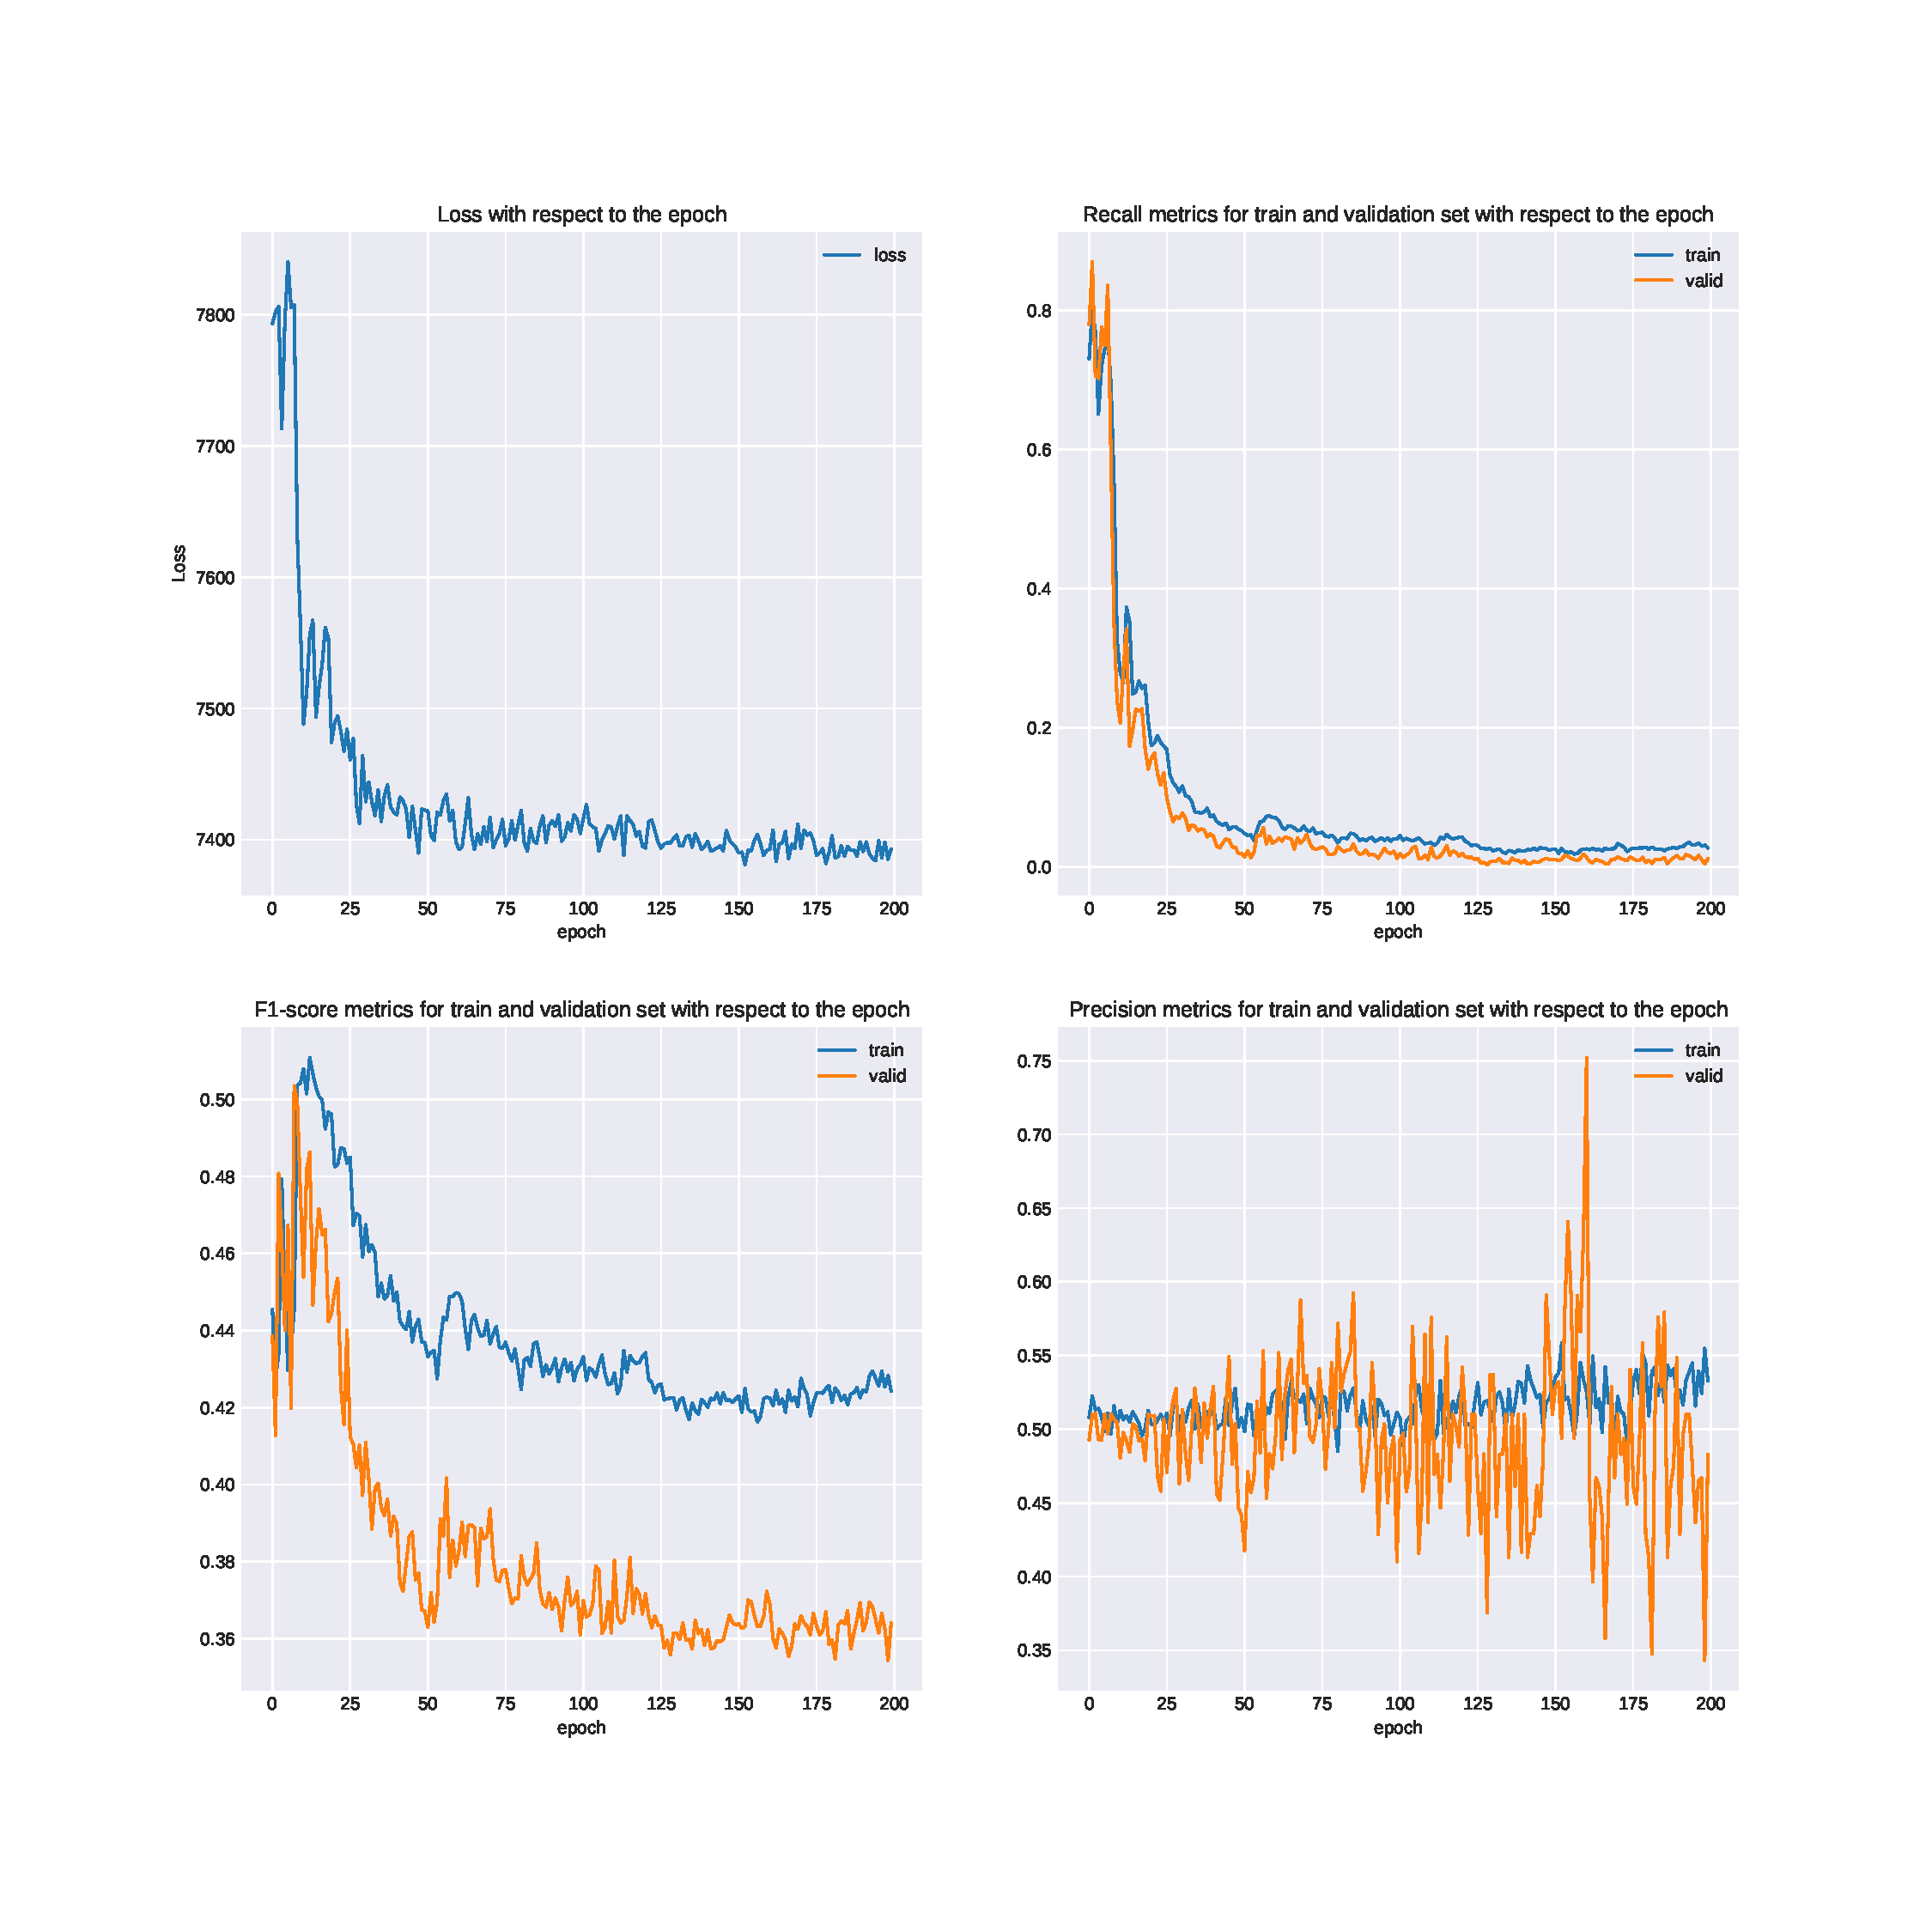
\includegraphics[width=0.8\textwidth]{images/chapitre4/appendix2_1.pdf}
	\caption{There is a spike for the precision, but that does not means that the model performs well.}
	\label{appendix2:training_plot1}
\end{figure}

\begin{figure}[h]
	\centering
	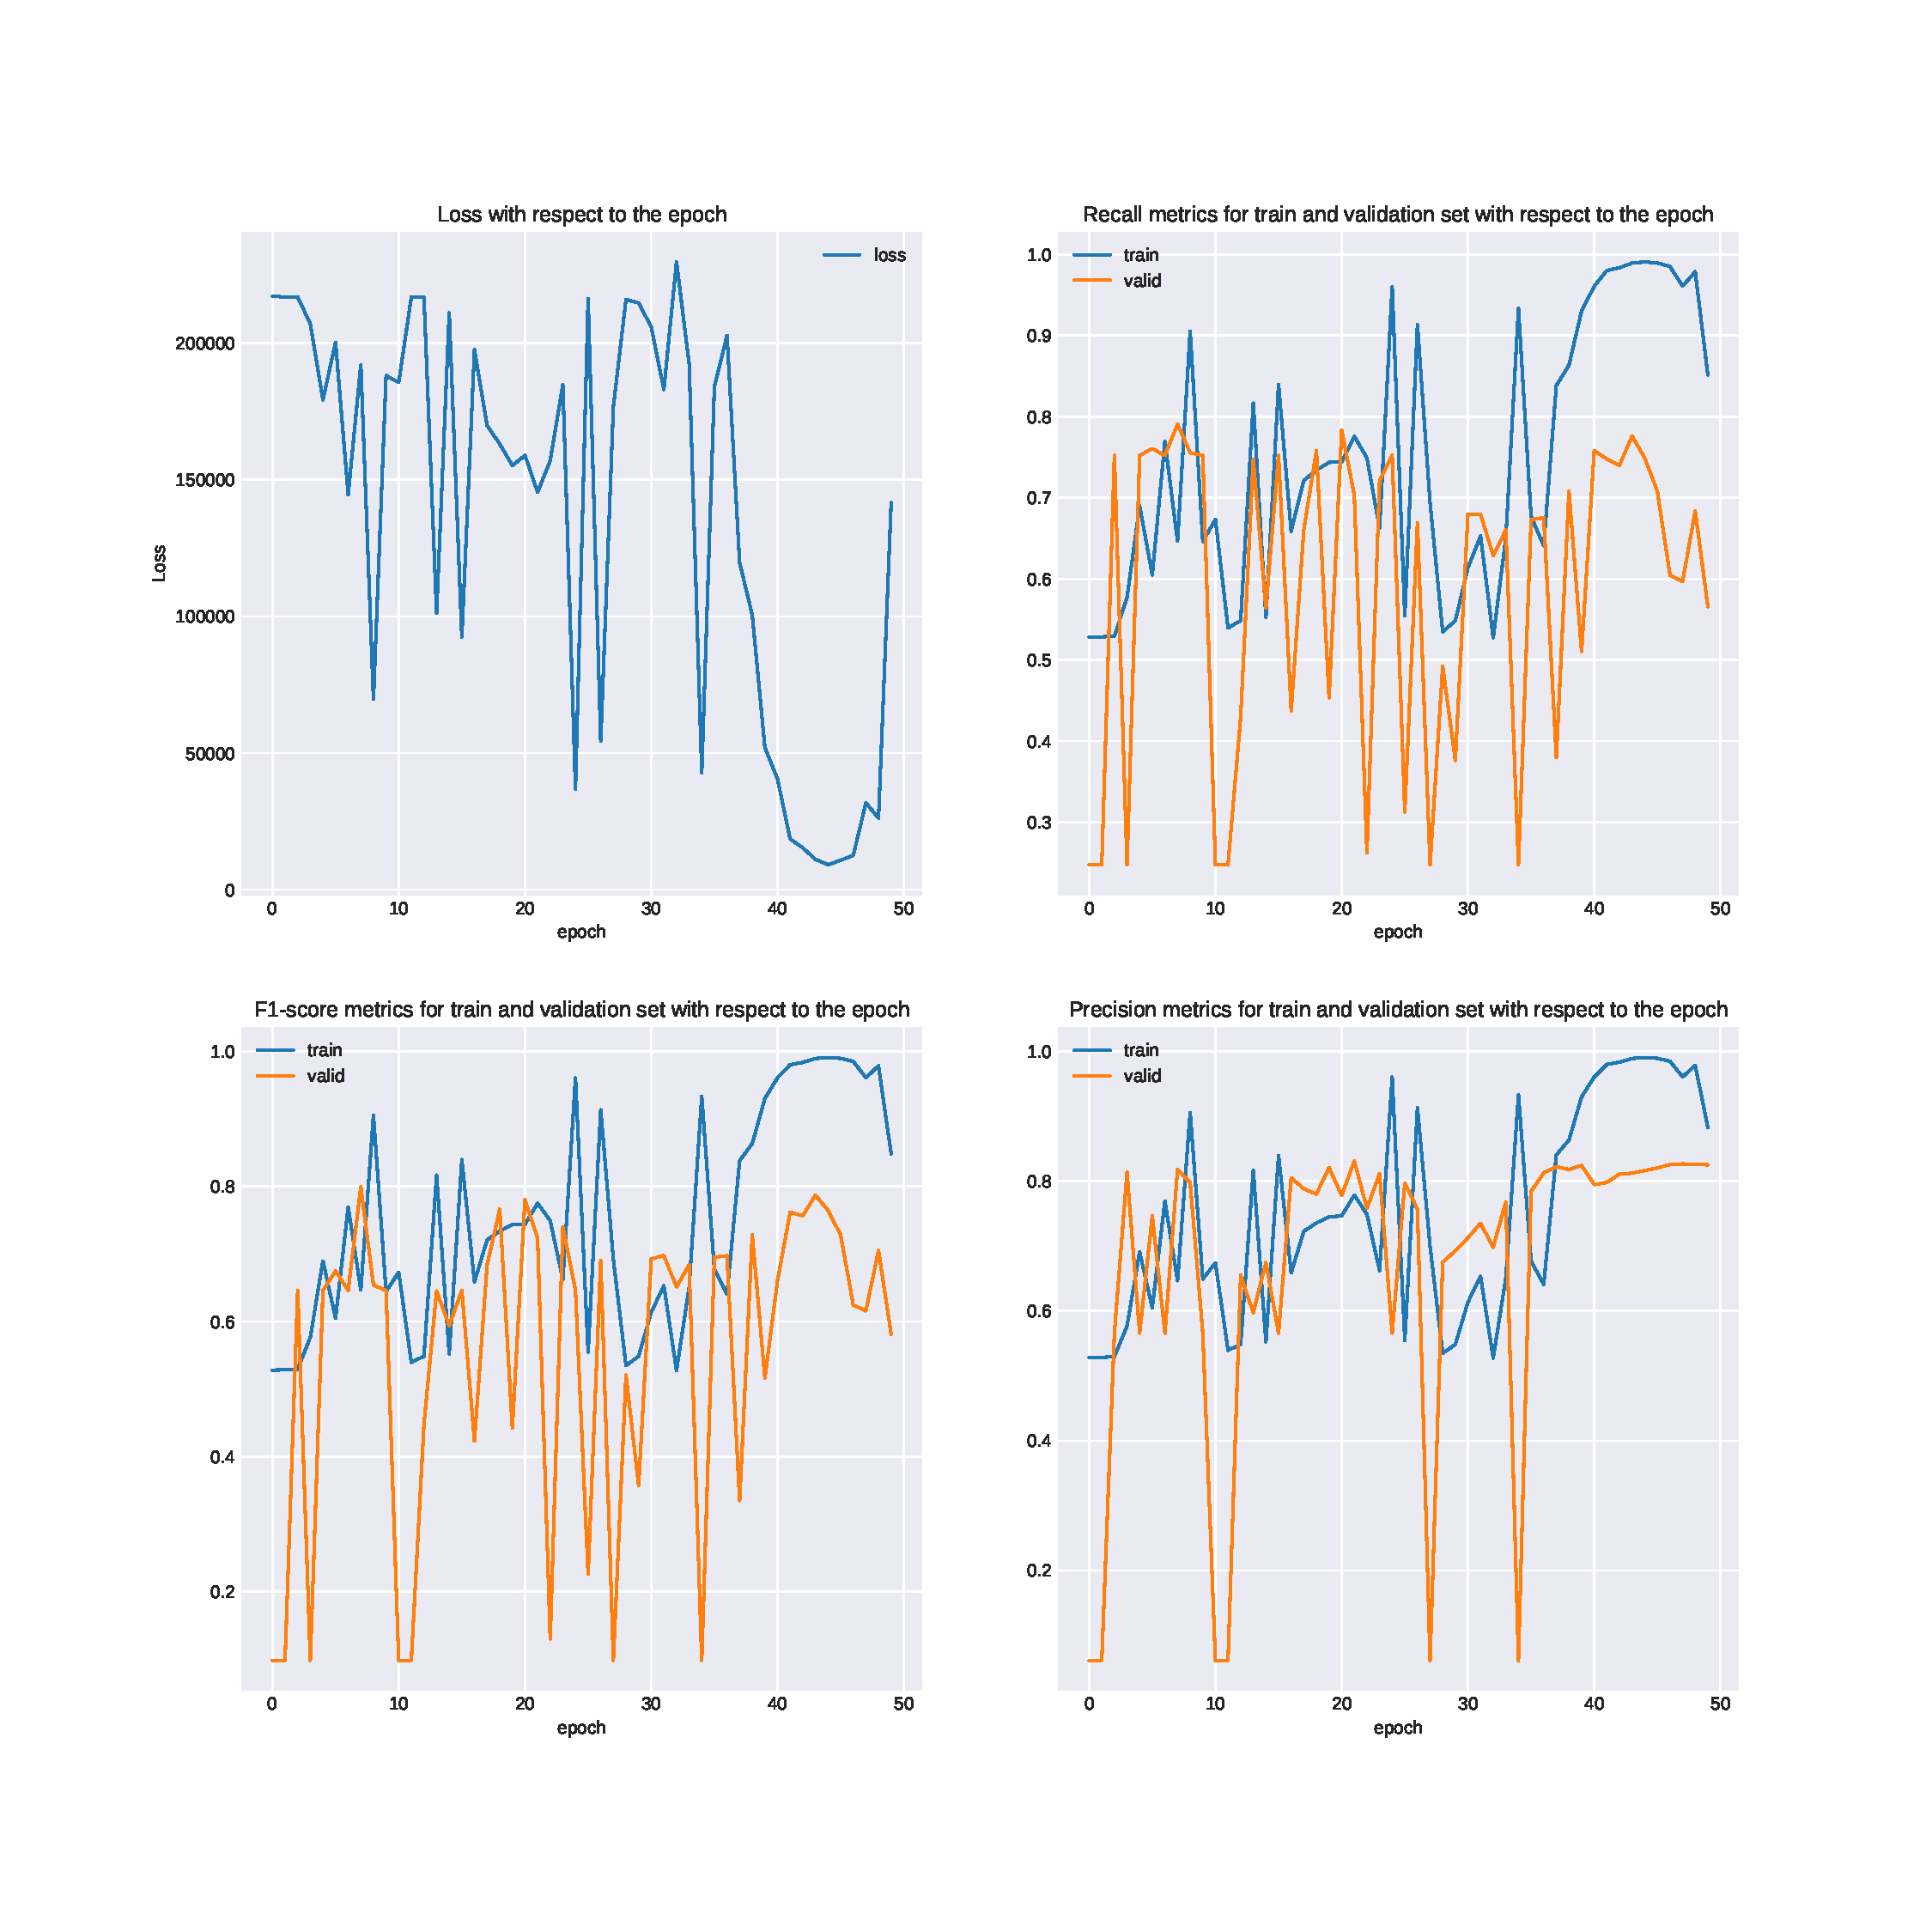
\includegraphics[width=0.8\textwidth]{images/chapitre4/attention5_2.pdf}
	\caption{Oscillation of the Loss}
	\label{appendix2:training_plot2}
\end{figure}
